\documentclass[a4paper]{article}
\usepackage{cmap}
\usepackage{mathtext}
\usepackage{amssymb}
\usepackage{amsmath}
\usepackage{wrapfig}
\usepackage[russian]{babel}
\usepackage{indentfirst}
\usepackage[pdftex]{graphicx}
\usepackage{multirow}
\usepackage{mathrsfs}
\usepackage{biblatex}
\usepackage{siunitx}
\usepackage[left=2cm,right=2cm,top=2cm,bottom=2cm]{geometry}
\usepackage{fancyhdr}
\bibliography{bib}
\pagestyle{fancy}
\newcommand{\const}{\mathrm{const}}
\newcommand{\rref}[1]{(\ref{#1})}
\newenvironment{comment}{}{}
\newcommand{\picref}[1]{рис. \ref{#1}}
\newcommand{\mbf}{\mathbf}
\newcommand{\Equip}[3]{
	
	\item{\bf #1:} $\Delta = \pm #2\; #3$}
\newcommand{\equip}[1]{
	
	\item{\bf #1}}
\newcommand{\labname}{Изучение рассеяния медленных электронов на атомах (эффект Рамзауэра)} 	% название пиши здесь
\newcommand{\labnum}{5.1.3}		% номер вводи здесь
\fancyfoot{}
\fancyhead[RE, RO]{\thepage}
\fancyhead[LE, LO]{Лабораторная работа \labnum \space \labname}
\title{Лабораторная работа \labnum \space \labname} % Название работы здесь
\author{Иван Сладков}
\begin{document}
\maketitle
\thispagestyle{empty}
\section{Аннотация}
В данной работе исследуется энергетическая зависимость вероятности рассеяния электронов атомами ксенона, определяются энергии электронов, при которых наблюдается <<просветление>> ксенона, и оценивается размер его внешней электронной оболочки.

\section{Теоретические сведения}

\begin{wrapfigure}{}{0.3\textwidth}
	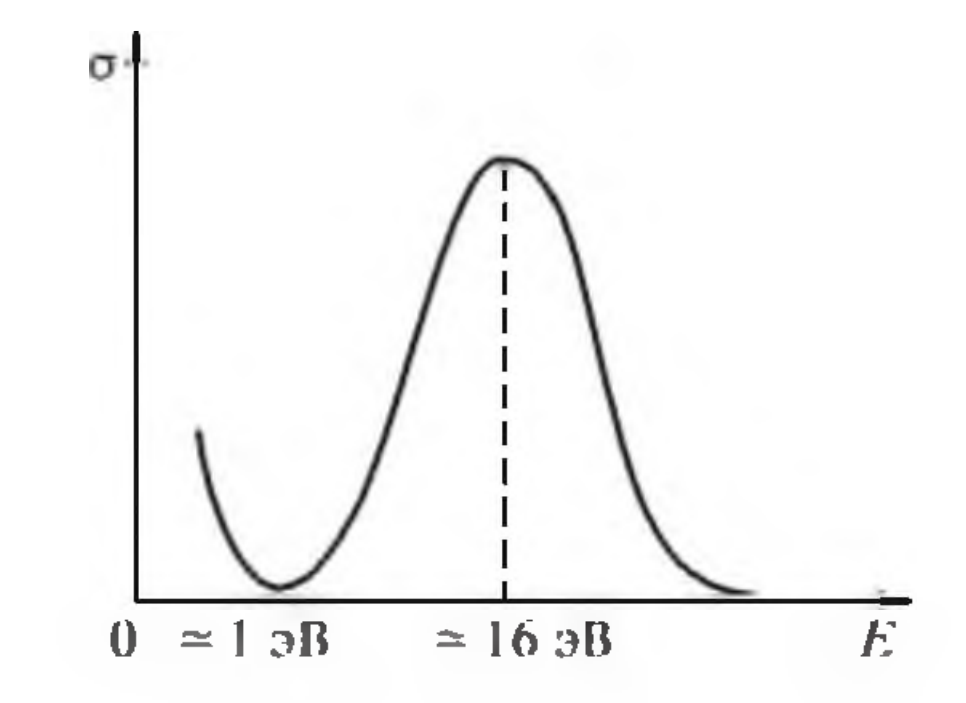
\includegraphics[width=1.0\linewidth]{Screenshot_1}
	\caption{Качественная картина результатов измерения упругого рассеяния электронов в аргоне}
	\label{fig:screenshot1}
\end{wrapfigure}
Эффективное сечение реакции -- это величина, характеризующая вероятность перехода системы двух сталкивающихся частиц в результате их рассеяния (упругого или неупругого) в определенное конечное состояние. Сечение $ \sigma $ равно отношению числа $ N $ таких переходов в единицу времени к плотности потока рассеиваемых частиц $ n v $, падающих на мишень, т. е. к числу частиц, проходящих в единицу времени через единичную площадку, перпендикулярную к их скорости $ v $ ($ n $ -- плотность числа падающих частиц).
\begin{equation}\label{eq:sigma}
	\sigma = \frac{N}{n v}.
\end{equation}
Таким образом, сечение имеет размерность площади.


\begin{figure}
	\centering
	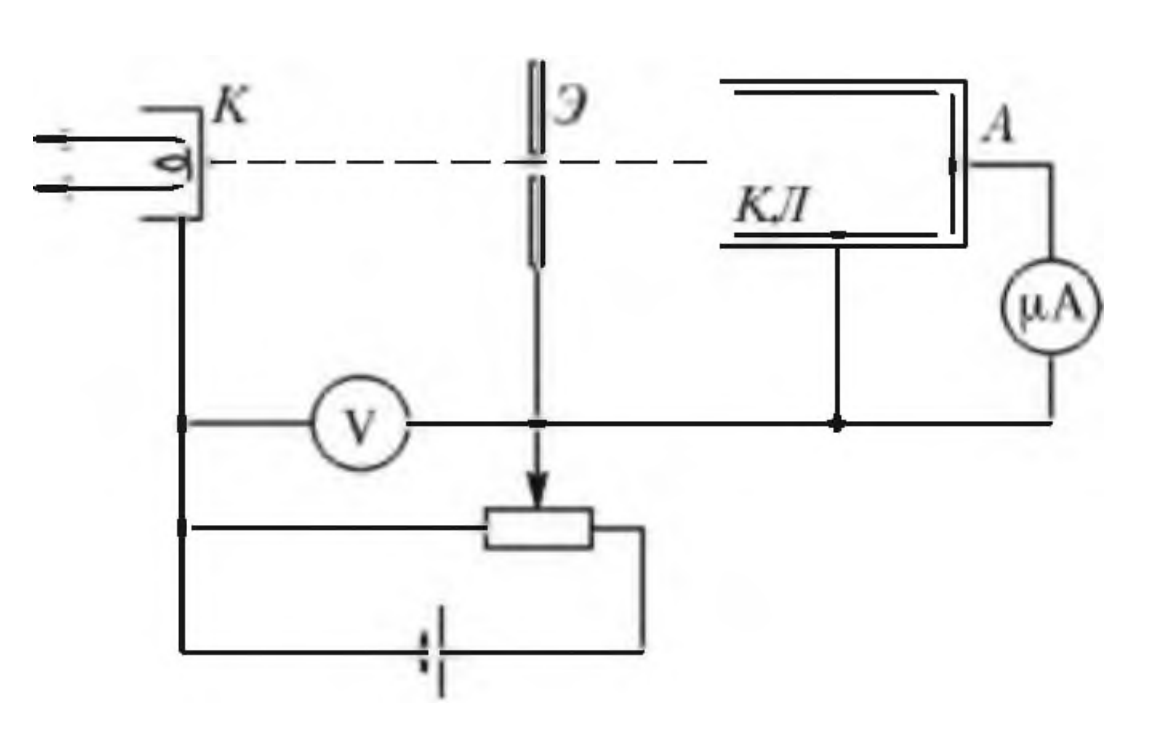
\includegraphics[width=0.5\linewidth]{Screenshot_2}
	\caption{Схема установки для измерения сечения рассеяния электронов в газах}
	\label{fig:screenshot2}
\end{figure}
Качественно результат экспериментов Рамзауэра при энергии электронов порядка десятков эВ показан на рис. \ref{fig:screenshot1}.
По мере уменьшения энергии электрона от нескольких десятков электрон-вольт поперечное сечение его упругого рассеяния растет. Однако при энергиях меньше 16 эВ в случае аргона сечение начинает уменьшаться, а при $ E \sim 1 $ эВ практически равно нулю, т. е. аргон становится прозрачным для электронов. При дальнейшем уменьшении энергии электронов сечение рассеяния опять начинает возрастать. Это поведение поперечного сечения свойственно не только атомам аргона, но и атомам всех инертных газов. Такое поведение электронов нельзя объяснить с позиций классической физики. Объяснение этого эффекта потребовало учета волновой природы электронов. Схема эксперимента Рамзауэра показана, на рис. \ref{fig:screenshot2}.


С точки зрения квантовой теории, внутри атома потенциальная энергия налетающего электрона $ U $ отлична от нуля, скорость электрона изменяется, становясь равной $ v' $ в соответствии с законом сохранения энергии
\begin{equation*}
	E = \frac{m v^2}{2} = \frac{m v'^2}{2}+ U,
\end{equation*}
а значит, изменяется и длина его волны де Бройля. Таким образом, по отношению к электронной волне атом ведет себя как преломляющая среда с относительным показателем преломления
\begin{equation*}
	n = \frac{\lambda}{\lambda'} = \sqrt{1-\frac{U}{E}}.
\end{equation*}

Коэффициент прохождения электронов максимален при условии
\begin{equation}\label{eq:at}
	\sqrt{\frac{2 m (E+U_0)}{\hbar^2}}l = \pi n;\; n \in \mathbb{N}_1,
\end{equation}
где $ U_0 $ -- глубина потенциальной ямы.

Это условие легко получить, рассматривая интерференцию электронных волн де Бройля в атоме. Движущемуся электрону соответствует волна де Бройля, длина которой определяется соотношением $ \lambda = h/m v $. Если кинетическая энергия электрона невелика, то $ E = m v^2/2 $ и $ \lambda = h/\sqrt{2 m E} $. При движении электрона через атом длина волны де Бройля становится меньше и равна $ \lambda' = h/\sqrt{2 m (E+U_0)} $ где $ U_0 $ — глубина атомного потенциала. При этом, волна де Бройля отражается от границ атомного потенциала, т. е. от поверхности атома, и происходит интерференция прошедшей через атом волны 1 и волны 2, отраженной от передней и задней границы атома (эти волны когерентны). Прошедшая волна 1 усилится волной 2, если геометрическая разность хода между ними $ \Delta = 2 l = \lambda' $, что соответствует условию первого интерференционного максимума, т. е. при условии
\begin{equation}\label{eq:condition}
	2 l = \frac{h}{\sqrt{2 m (E_1 + U_0)}}
\end{equation}
Прошедшая волна ослабится при условии
\begin{equation}\label{eq:condition2}
	2 l = \frac{3}{2}\frac{h}{\sqrt{2 m (E_1 + U_0)}}
\end{equation}

Из \eqref{eq:condition} и \eqref{eq:condition2}, можно получить
\begin{equation}\label{eq:radius}
	l = \frac{h \sqrt{5}}{\sqrt{32 m (E_2-E_1)}}.
\end{equation}
Оттуда же можно найти эффективную глубину потенциальной ямы атома:
\begin{equation}\label{eq:atomPit}
	U_0 = \frac{4}{5}E_2-\frac{9}{5} E_1.
\end{equation}

\subsection{Расчётные формулы}

Уравнение вольт-амперной характеристики тиратрона:
\begin{equation}\label{eq:VAH}
	I_а = I_0 \exp (-C \omega (V));\; C = L n_а \Delta_а,
\end{equation}
где $ I_0 = e N_0 $ -- ток катода, а $ I_а = e N_а $ -- ток анода.
Отсюда определяется вероятность рассеяния электрона в зависимости от его энергии:
\begin{equation}\label{eq:probable}
	\omega (V) = -\frac{1}{C} \ln \frac{I_а(V)}{I_0}.
\end{equation}
\section{Оборудование и инструментальные погрешности}

Схема экспериментальной установки отображена на рис. \ref{fig:screenshot3}.
\begin{figure}
	\centering
	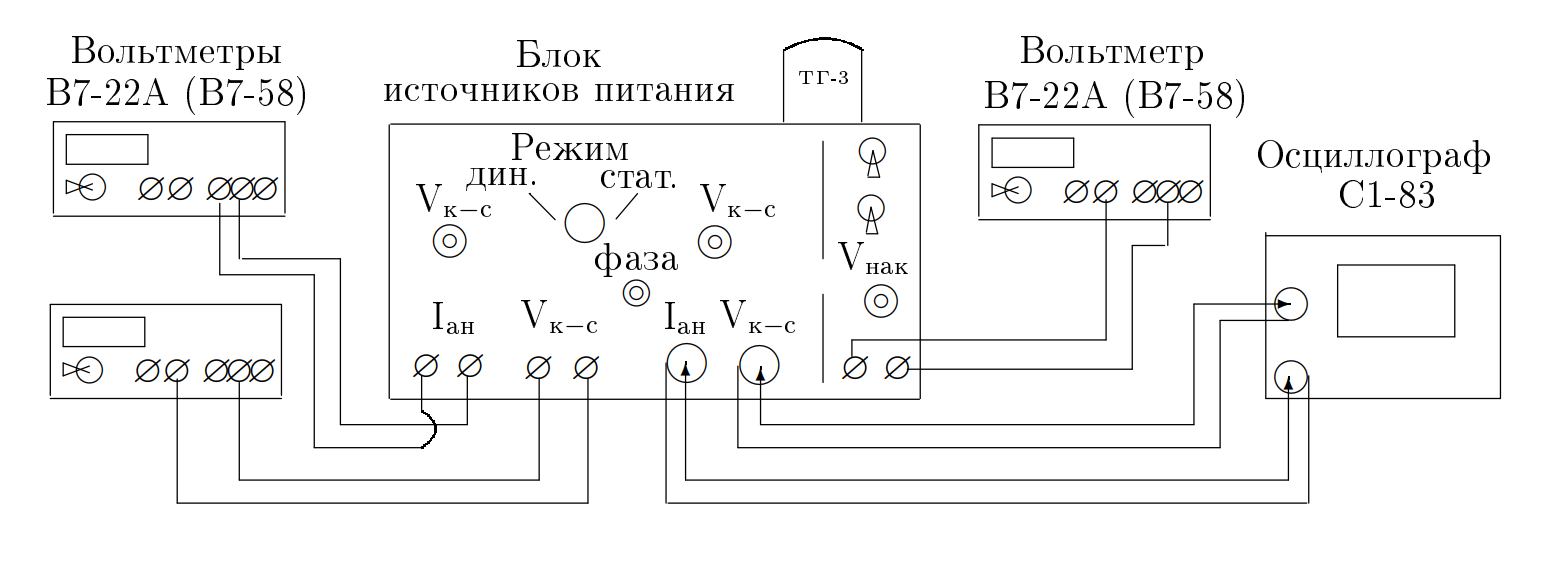
\includegraphics[width=1.0\linewidth]{Screenshot_3}
	\caption{Схема экспериментальной установки}
	\label{fig:screenshot3}
\end{figure}
В данной работе для изучения эффекта Рамзауэра используется
тиратрон ТГЗ-01/1.3Б, заполненный инертным газом. Электроны, эмитируемые катодом тиратрона, ускоряются напряжением $ V $, приложенным между катодом и ближайшей к нему сеткой. Затем электроны рассеиваются на атомах инертного газа (ксенона). Все сетки соединены между собой и имеют одинаковый потенциал, примерно равный потенциалу анода. Поэтому между первой сеткой и анодом практически нет поля. Рассеянные электроны отклоняются в сторону и уходят на сетку, а оставшаяся часть электронов достигает анода и создаёт анодный ток $ I_а $. Таким образом, поток электронов $ N(x) $ (т. е. число электронов, проходящих через поперечное сечение лампы в точке $ x $ в единицу времени) уменьшается с ростом $ x $ от начального значения $ X $ y катода (в точке $ x=0 $) до некоторого значения $ N_а $ у анода (в точке
$ x=L $).


В работе используются:
\begin{itemize}
	\Equip{Вольтметры}{0.01}{В}
	\Equip{Осциллограф}{0.2}{В} по оси X
	\equip{Блок источников питания}
	\equip{Тиратрон ТГ3}
\end{itemize}

\section{Результаты измерений и обработка данных}
\emph{Все измерения и расчёты в СИ.}

\subsection{Динамический метод}

По результатам измерений в динамическом режиме оценим размер электронной оболочки атома инертного газа по формулам \eqref{eq:condition} и \eqref{eq:condition2}. 
Положение первого максимума $$ V_{max}^1 \approx 2.5 \;В.$$
Положение первого минимума $$ V_{min}^1 \approx 6.5 \; В.$$
Тогда 
\begin{equation*}\label{key}
	l = \frac{h}{\sqrt{2 m_e * 5}} \approx 2.8\; \text{\AA{}}
\end{equation*}
\begin{equation*}
	l = \frac{3}{4} \frac{h}{\sqrt{2 m_e * 9}} \approx 3\; \text{\AA{}}
\end{equation*}
В данном случае оценка погрешностей не имеет смысла, так как точка $ V_{max}^1 $ указана неточно, а сам расчёт носит оценочный характер.

Далее найдём радиус из формулы \eqref{eq:radius}:
\begin{equation*}\label{key}
	l = (3.4 \pm 0.2)*10^{-10} \; \text{\AA{}}
\end{equation*}

Эффективная глубина потенциальной ямы равна
\begin{equation*}\label{key}
	U_0 = \frac{4}{5}*6.5 - \frac{9}{5}*2.5 = 1.1 \;эВ.
\end{equation*}

Так как напряжение пробоя примерно равно $ 12  $ В, в колбу закачан ксенон. Установить напряжение пробоя более точно не удалось, так как даже при $ V_{накала} = 3.3 $ В не наблюдалось достаточно резкого возрастания тока анода, то есть было сложно найти конкретную точку $ V_{пробоя}. $

\subsection{Статический метод}

По результатам статического измерения, получены данные табл. \ref{tab:ВАХ}. По этим данным построим графики на рис. \ref{fig:v--2} и \ref{fig:v--3}. Для графика \ref{fig:v--3} проведём дополнительный анализ на пики.

\begin{figure}
	\centering
	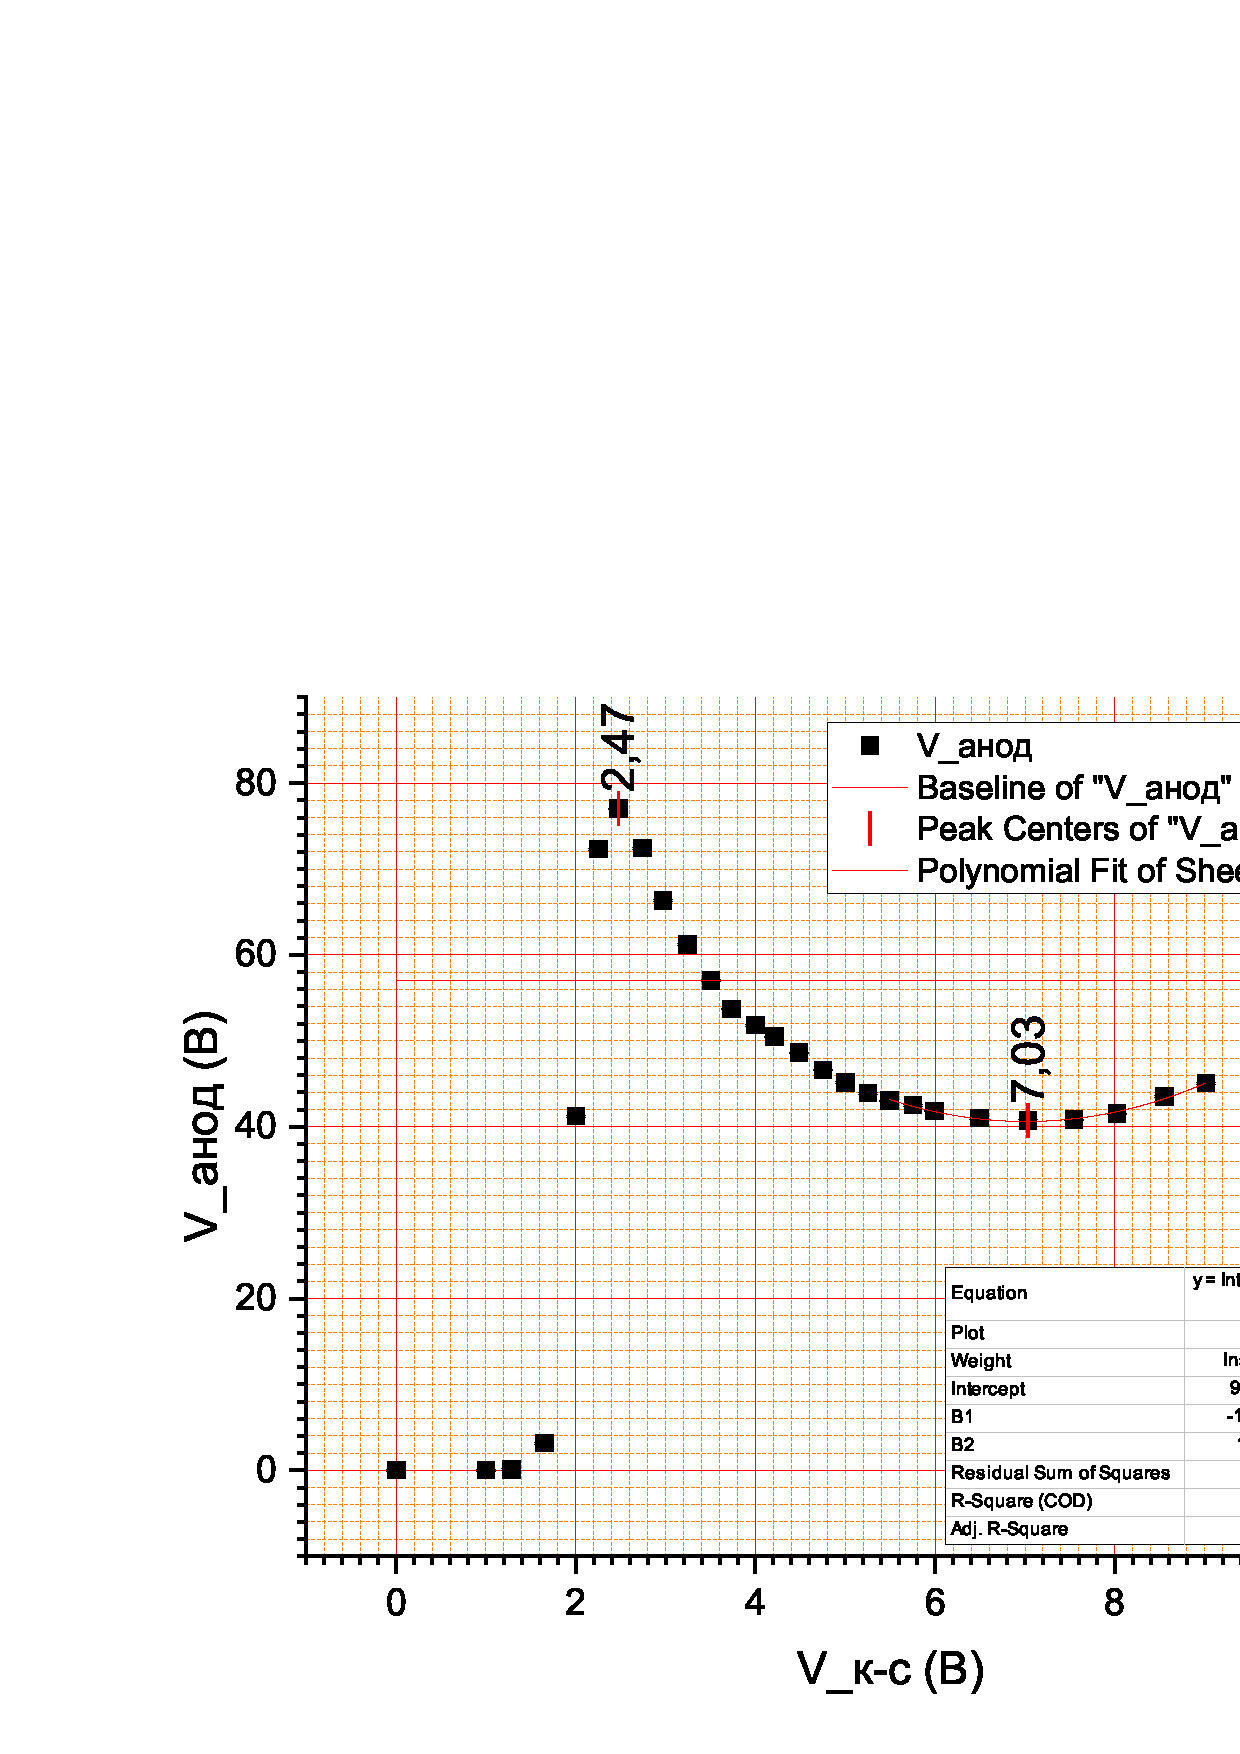
\includegraphics[width=1.0\linewidth]{V1}
	\caption{Вольт-амперная характеристика при $V_{накала} = 2.99 \; В$}
	\label{fig:v--2}
\end{figure}


\begin{figure}
	\centering
	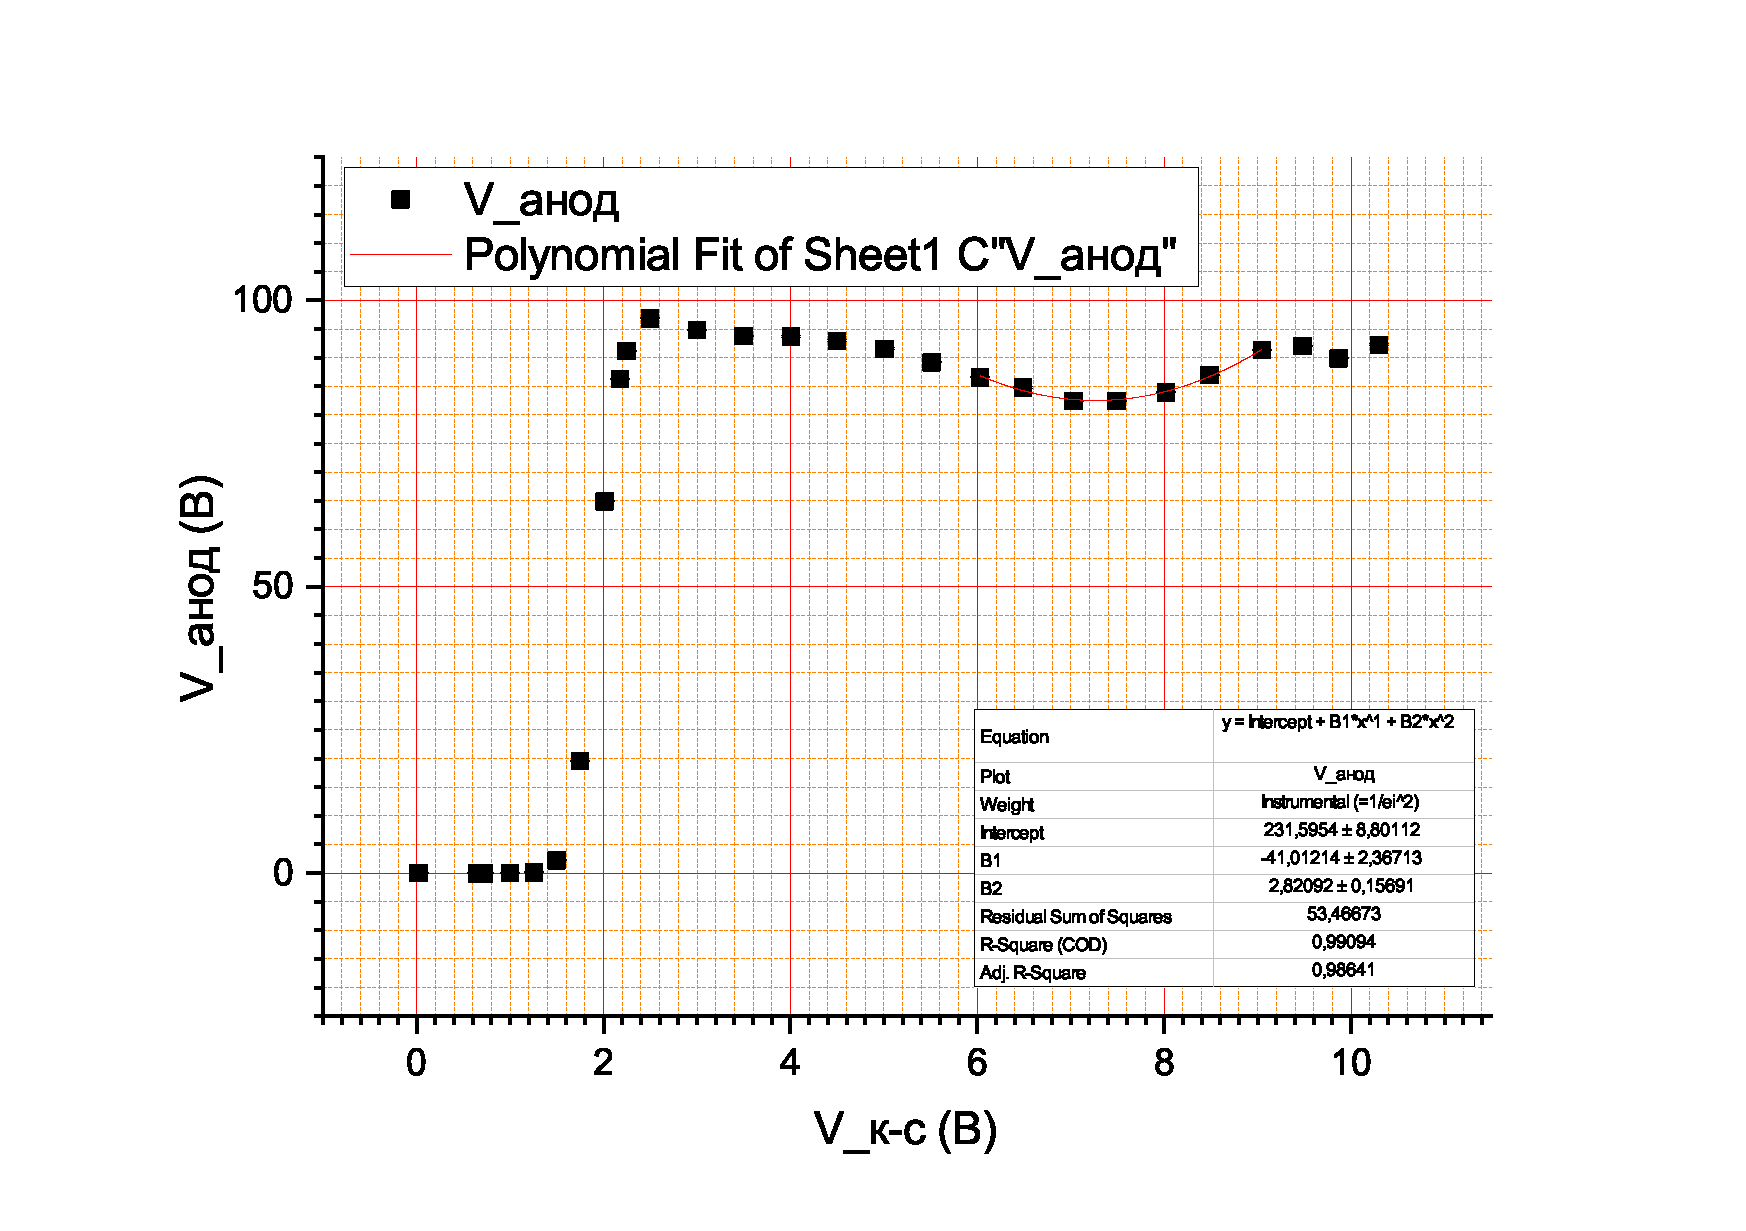
\includegraphics[width=1.0\linewidth]{V2}
	\caption{Вольт-амперная характеристика при $V_{накала} = 3.31 \; В$}
	\label{fig:v--3}
\end{figure}

\begin{table}[]
	\centering
	\begin{tabular}{|l|l|l|}
		\hline
		n                       & $V_1$        & $V_2$        \\ \hline
		$V_{накала} = 3.31\; В$ & $2.3\pm 0.2$ & $7.3\pm 0.6$ \\ \hline
		$V_{накала} = 2.99\; В$ & $2.5\pm 0.2$ & $7.0\pm 0.6$ \\ \hline
	\end{tabular}
	\caption{Результат опыта в статическом методе}
	\label{tab:stat}
\end{table}
По результатам, приведённым в табл.\ref{tab:stat},
\[
	l = (3.1 \pm 0.3)*10^{-10} \; \text{\AA{}}.
\]
Глубина потенциальной ямы
\[
	U_0 = 1.7\pm 0.1.
\]

Далее по формуле \eqref{eq:at} оценим, при каких напряжениях должны появляться максимумы в коэффициенте прохождения электронов:
\[
	E = \sqrt{\frac{\pi n \hbar}{l}} \frac{1}{2 m} - U_0,
\]
\[  E_{n=2}= 15 \pm 1 \; эВ,\]
\[  E_{n=3} = 31 \pm 2 \; эВ. \]
Эти максимумы никак не отображаются на графике, так как они больше потенциала ионизации, при достижении которого картина кардинально меняется.

Далее, по формуле \eqref{eq:probable} найдём зависимость вероятности рассеяния от энергии
\[\omega(V) \propto \ln \frac{V_{анод}}{V_{анод}^0},\] где $ V_{анод}^0 $ -- первый максимум на ВАХ тиратрона. Результат отображён на рис. \ref{fig:graph4}. Заметим, что на рис. отображена зависимость не для $ \ln I/I_0 $, а для $ \ln V/V_0 $, что в общем не имеет значения.

\begin{figure}
	\centering
	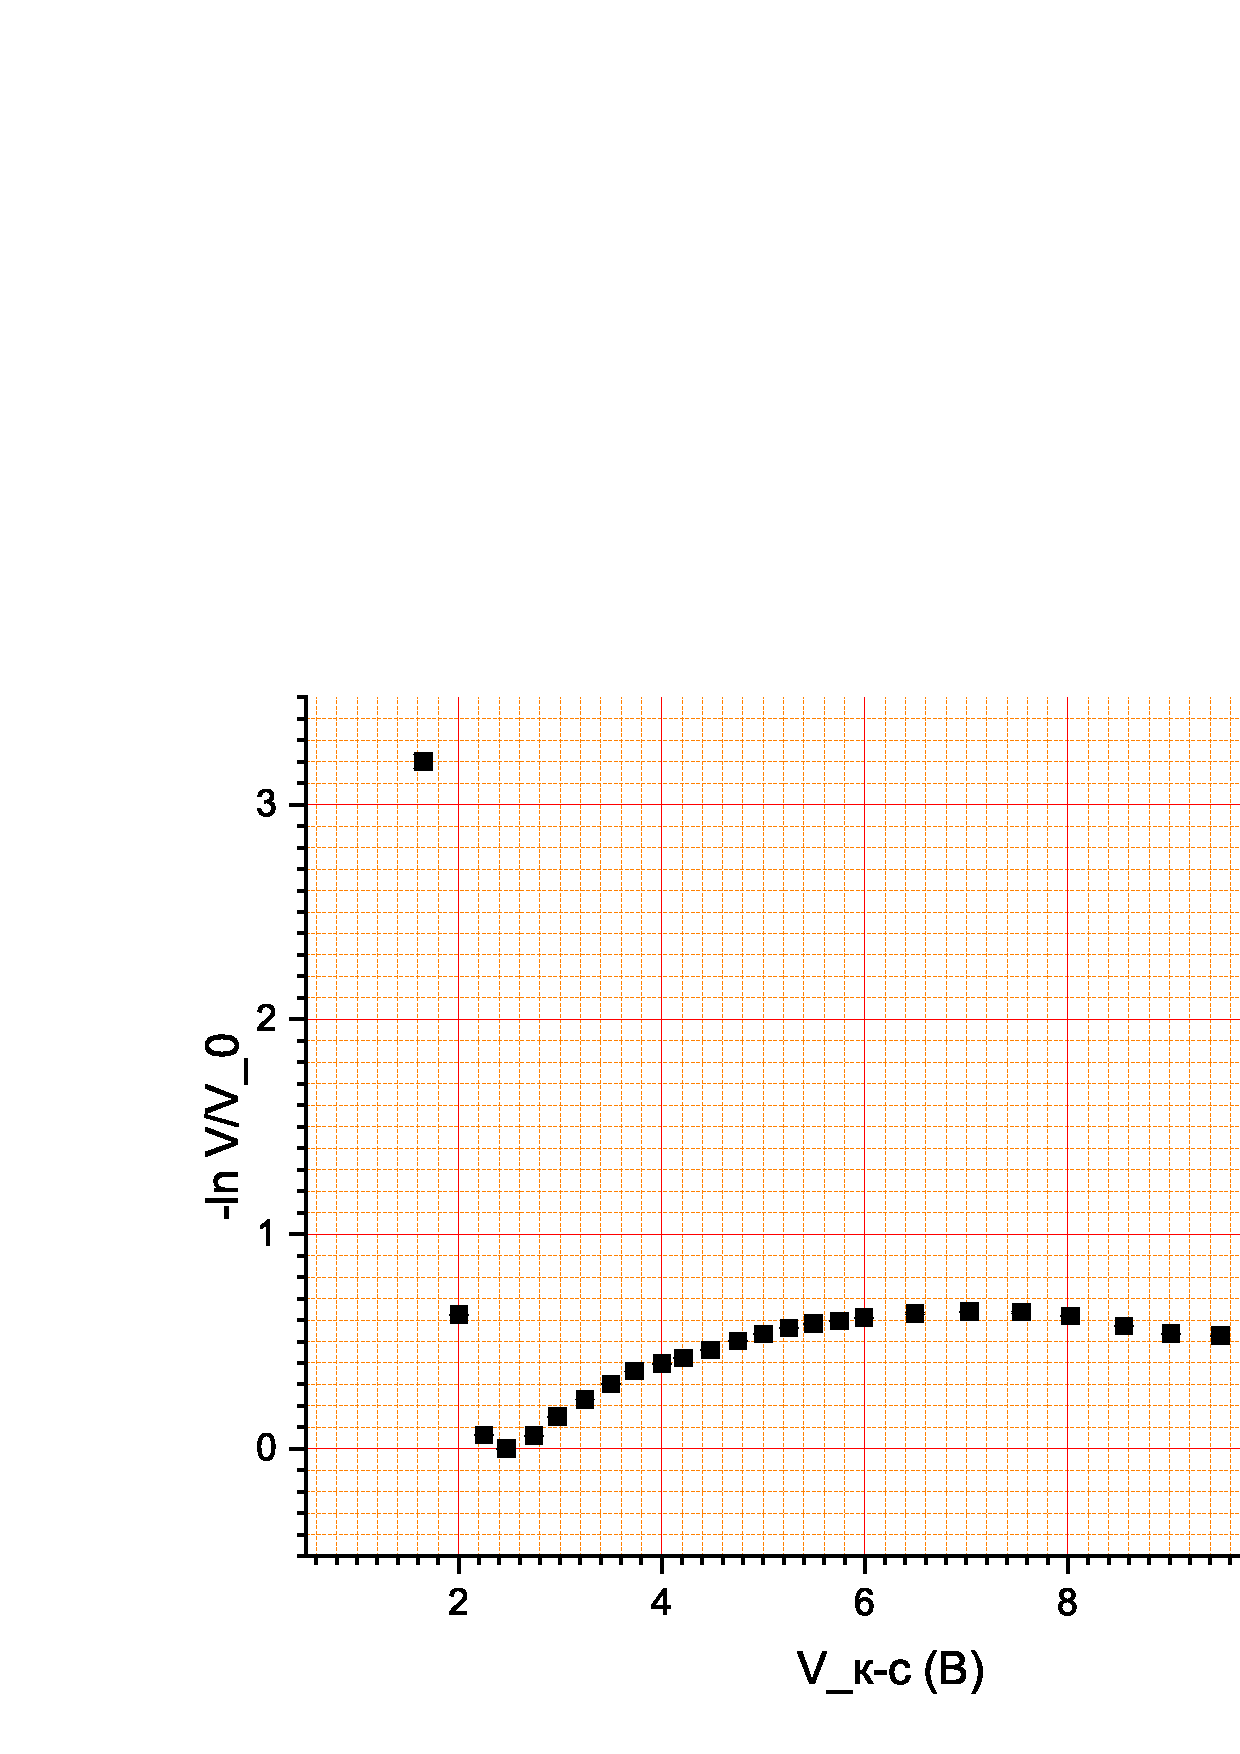
\includegraphics[width=1.0\linewidth]{Graph5}
	\caption{Качественный график зависимости $ \omega \propto -\ln \frac{I}{I_0} = F(V) $}
	\label{fig:graph4}
\end{figure}

\section{Вывод}

По результатам проведения лабораторной работы установлен приблизительный радиус атома ксенона, эффективная глубина потенциальной ямы для электрона, а также получен график зависимости $ \omega = F(E) $ для вероятности рассеяния электрона. Исходя из полученных данных, результат статического измерения точнее. Отчасти это может быть связано с некоторой инерционностью происходящих в тиратроне процессов: например, время установления картины на осциллографе исчисляется секундами, что может говорить об инерционности других процессов.

\appendix
\section{Необработанные результаты опытов}

<<Сырые>> данные по результатам опыта представлены в табл. \ref{tab:ВАХ}.

\begin{table}[]
	\centering
	\begin{tabular}{|l|l|l|l|}
		\hline
		\multicolumn{2}{|l|}{$V_{накал}  = $ 3.31 В} & \multicolumn{2}{l|}{$V_{накал}  = $ 2.99 В} \\ \hline
		$V_{катод}$, В        & $V_{анод}$, В        & $V_{катод}$, В        & $V_{анод}$, В       \\ \hline
		0,02  & 0,04  & 10,9 & 60    \\ \hline
		10,3  & 92,3  & 9,5  & 45,5  \\ \hline
		9,87  & 89,9  & 9,01 & 45,04 \\ \hline
		9,48  & 92,1  & 8,55 & 43,5  \\ \hline
		9,05  & 91,4  & 8,02 & 41,5  \\ \hline
		8,49  & 87    & 7,54 & 40,8  \\ \hline
		8,02  & 84    & 7,03 & 40,7  \\ \hline
		7,49  & 82,5  & 6,49 & 41    \\ \hline
		7,03  & 82,5  & 5,99 & 41,82 \\ \hline
		6,49  & 84,8  & 5,75 & 42,51 \\ \hline
		6,03  & 86,6  & 5,49 & 43    \\ \hline
		5,51  & 89,2  & 5,25 & 43,9  \\ \hline
		5,01  & 91,6  & 5    & 45,12 \\ \hline
		4,5   & 93    & 4,75 & 46,6  \\ \hline
		4,01  & 93,7  & 4,48 & 48,6  \\ \hline
		3,5   & 93,8  & 4,21 & 50,45 \\ \hline
		3     & 94,87 & 4    & 51,8  \\ \hline
		2,5   & 96,87 & 3,73 & 53,7  \\ \hline
		2,01  & 64,9  & 3,5  & 57    \\ \hline
		2,18  & 86,3  & 3,24 & 61,2  \\ \hline
		2,25  & 91,2  & 2,97 & 66,3  \\ \hline
		1,75  & 19,6  & 2,74 & 72,4  \\ \hline
		1,5   & 2,22  & 2,47 & 77    \\ \hline
		1,26  & 0,18  & 2,25 & 72,3  \\ \hline
		1     & 0,02  & 2    & 41,2  \\ \hline
		0,723 & 0     & 1,65 & 3,14  \\ \hline
		0,647 & 0     & 1,28 & 0,06  \\ \hline
		---   & ---   & 1    & 0,01  \\ \hline
		---   & ---   & 0    & 0     \\ \hline
	\end{tabular}
	\caption{Данные по ВАХ тиратрона}
	\label{tab:ВАХ}
\end{table}

\begin{thebibliography}{9}
	\bibitem{Siv} Сивухин Д. В. \emph{Общий курс физики. Том 4 Оптика}, 2004
	\bibitem{kir} Кириченко Н. А. \emph{Принципы оптики}, 2014
	\bibitem{max} \emph{Лабораторный практикум по общей физике. В 3 томах. Том 2. Оптика: учебное пособие} под ред. А. В. Максимычева
\end{thebibliography}
\end{document}